\documentclass[class=report, crop=false]{standalone}
\usepackage[subpreambles=true]{standalone}

\begin{document}
    \section{Resultatet}
    Efter kørslen af programmerne kunne vi sammenligne resultaterne, som kan ses herunder. Det ses at C\# programmet kører betydeligt hurtigere end Python programmet.\\
    Resultatets middelværdi lå meget højere i Python, som vi havde forventet, men udover dette er differencen også en del højere, som vi ikke havde forventet. Ved at skrive alle gennemsnitsværdierne ud i stedet for middelværdien, kunne vi plotte de to programmer, som kan ses på Figur \ref{fig:SpeedPlot}. Dette gav et tydeligt indblik i stabiliteten af de to sprog, som viser at Python kører meget mere ustabilt også.

    \begin{tcolorbox}
        \text{C\#: } \[ 311,2 \text{ ns} \pm 13,1  \]
    \end{tcolorbox}
    \begin{tcolorbox}
        \text{Python: } \[ 3312,1 \text{ ns} \pm 88,9  \]
    \end{tcolorbox}

    \begin{tcolorbox}
        \begin{figure}[H]
            \centering
            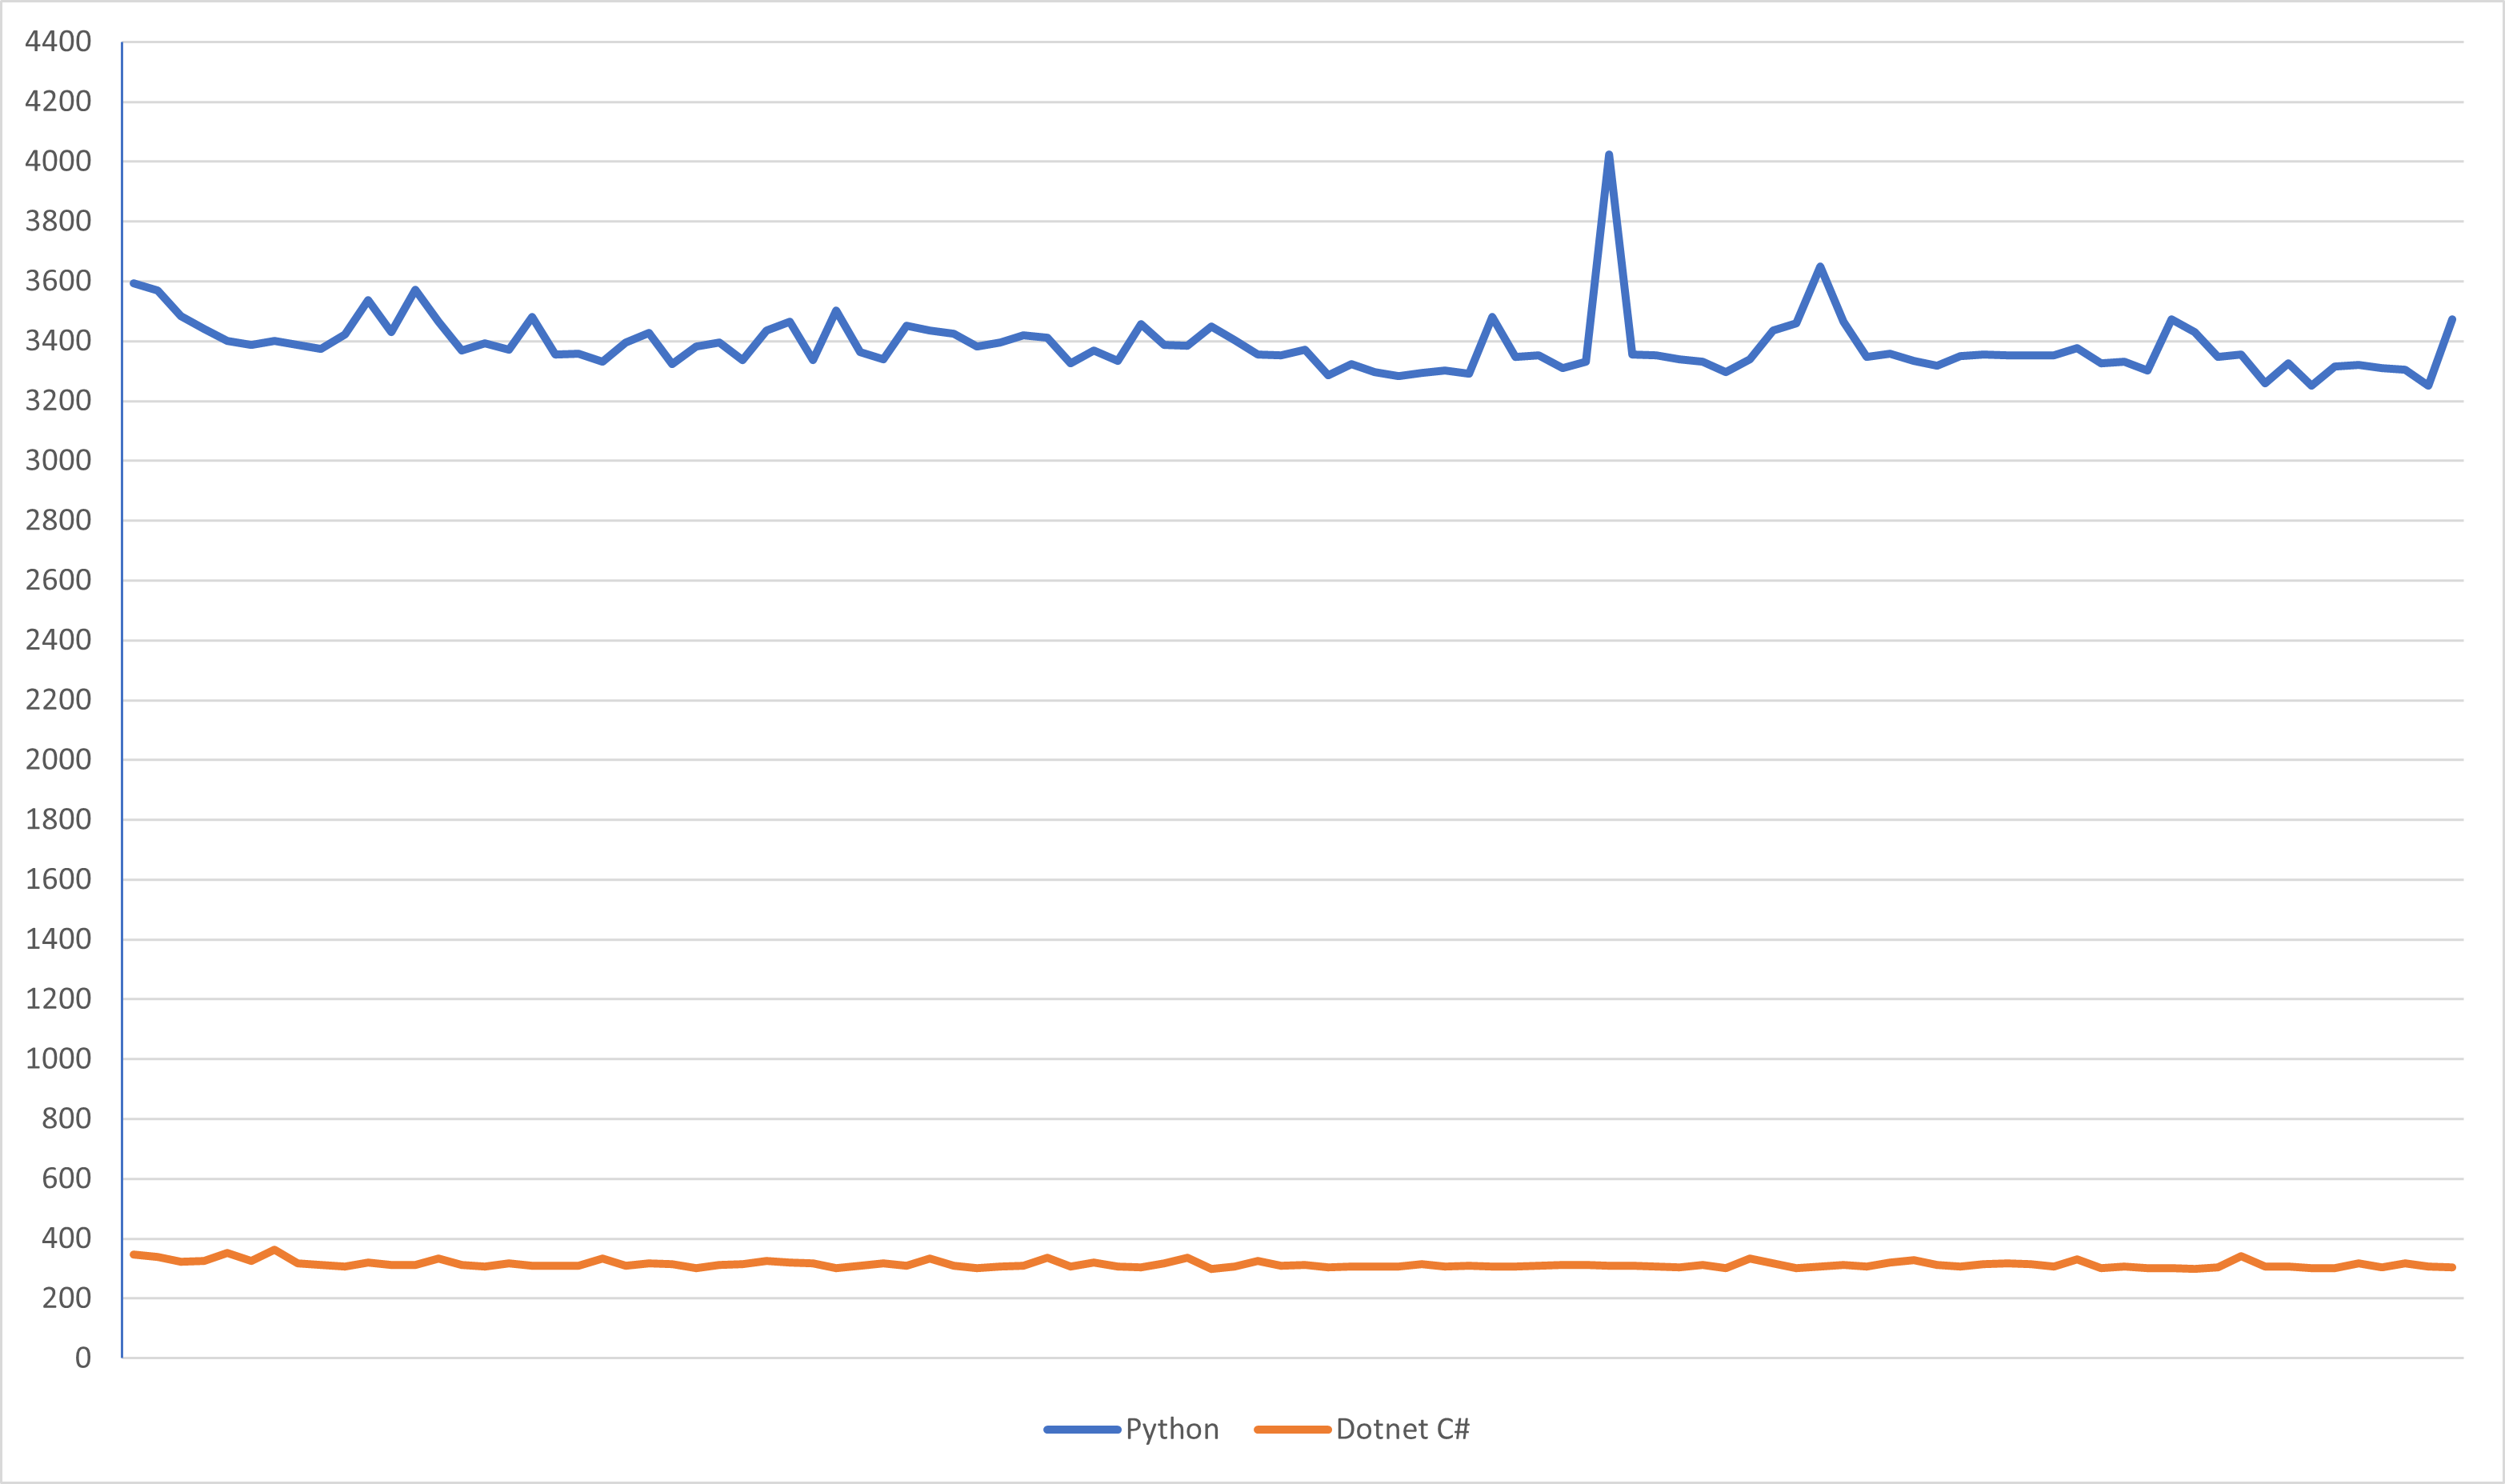
\includegraphics[width=\textwidth]{SpeedPlot.png}
            \caption{Plot af hastighed på Insertion Sort}
            \label{fig:SpeedPlot}
        \end{figure}
    \end{tcolorbox}

\end{document}